\documentclass[9pt,aspectratio=169,xcolor=table]{beamer}

%~~~~~~~~~~~~~~~~~~~~~~~~~~~~~~~~~~~~~~~~~~~~~~~~~~~~~~~~~~~~~~~~~~~~~~~~~~~~~~
% Use roboto Font (recommended)
\usepackage[sfdefault]{roboto}
\usepackage[utf8]{inputenc}
\usepackage[T1]{fontenc}
%~~~~~~~~~~~~~~~~~~~~~~~~~~~~~~~~~~~~~~~~~~~~~~~~~~~~~~~~~~~~~~~~~~~~~~~~~~~~~~

%~~~~~~~~~~~~~~~~~~~~~~~~~~~~~~~~~~~~~~~~~~~~~~~~~~~~~~~~~~~~~~~~~~~~~~~~~~~~~~
% Define where theme files are located. ('/styles')
\usepackage{styles/fluxmacros}
\usefolder{styles}
% Use Flux theme v0.1 beta
% Available style: asphalt, blue, red, green, gray
\usetheme[style=hunter]{flux}
%~~~~~~~~~~~~~~~~~~~~~~~~~~~~~~~~~~~~~~~~~~~~~~~~~~~~~~~~~~~~~~~~~~~~~~~~~~~~~~

%~~~~~~~~~~~~~~~~~~~~~~~~~~~~~~~~~~~~~~~~~~~~~~~~~~~~~~~~~~~~~~~~~~~~~~~~~~~~~~
% Extra packages
\usepackage{booktabs}
\usepackage{colortbl}
\usepackage{ragged2e}
\usepackage{amssymb}
\usepackage{multirow}
\usepackage{tikz}
\usetikzlibrary{arrows.meta, positioning, fit, backgrounds, calc, decorations.pathreplacing}
\setbeamertemplate{itemize items}[square]
\usepackage[scaled=.8]{beramono}
\usepackage{listings}
\usepackage{styles/lstlangarm}
\usepackage{array}
\usepackage{makecell}
\definecolor{bgcolor}{HTML}{F2E9E9}
% lstlangarm.sty references \color{mauve} for string literals but never defines
% it -- only fires when a listing contains a string. Define it here.
\definecolor{mauve}{rgb}{0.58,0,0.82}
% lstlangarm's C style sets commentstyle=green!20, which is unreadable on the
% pink listing background. Darken it globally.
\lstset{commentstyle=\color{green!45!black}}
% ragged-right fixed-width column -- must be defined in the preamble, never
% inside a frame (\newcolumntype's #1 breaks beamer's frame scanner)
\newcolumntype{R}[1]{>{\RaggedRight\arraybackslash}p{#1}}
%~~~~~~~~~~~~~~~~~~~~~~~~~~~~~~~~~~~~~~~~~~~~~~~~~~~~~~~~~~~~~~~~~~~~~~~~~~~~~~
% Table striping: odd rows white, even rows very light gray.
% Needs \documentclass[...,xcolor=table]{beamer} (beamer loads xcolor itself,
% so the option must go on the class, not \usepackage).
\definecolor{stripe}{gray}{0.94}
% \striped makes body rows alternate white, gray, white, ... starting white.
% \rowcolors counts from the first coloured body row; the header is not counted.
\newcommand{\striped}{\rowcolors{1}{white}{stripe}}
%~~~~~~~~~~~~~~~~~~~~~~~~~~~~~~~~~~~~~~~~~~~~~~~~~~~~~~~~~~~~~~~~~~~~~~~~~~~~~~

%~~~~~~~~~~~~~~~~~~~~~~~~~~~~~~~~~~~~~~~~~~~~~~~~~~~~~~~~~~~~~~~~~~~~~~~~~~~~~~
% TikZ block styles -- matches ch1/ch2
% Colour variables are named identically in the book's stm32primer.tex, so any
% tikzpicture using only the \tikzset{...} styles below can be copied verbatim
% between slides and book. Only the \definecolor/\colorlet VALUES differ: the
% book is printed, so it keeps every stroke pure black with muted fills. These
% slides are projected, so both fill AND stroke are bright and saturated to
% grab attention -- see stm32primer.tex for the print palette.
\definecolor{blkfill}{HTML}{DDEEDD}
\definecolor{blkline}{HTML}{355E3B}
\definecolor{accentfill}{HTML}{FFE0B2}
\definecolor{accentline}{HTML}{E65100}
\definecolor{memfill}{HTML}{DFF5DA}
\definecolor{memline}{HTML}{2E7D32}
\definecolor{cellfill}{HTML}{FFFFFF}
\definecolor{cellline}{HTML}{424242}
\definecolor{bitmaskfill}{HTML}{DCEBFF}
\definecolor{bitmaskline}{HTML}{1565C0}
\definecolor{bithitfill}{HTML}{FFE0B2}
\definecolor{bithitline}{HTML}{E65100}
\tikzset{
  blk/.style   = {rectangle, rounded corners=2pt, draw=blkline, fill=blkfill,
                  thick, align=center, font=\small, minimum height=9mm, inner sep=3pt},
  cpublk/.style= {rectangle, rounded corners=2pt, draw=accentline, fill=accentfill,
                  thick, align=center, font=\small\bfseries, minimum height=9mm, inner sep=3pt},
  memblk/.style= {rectangle, rounded corners=2pt, draw=memline, fill=memfill,
                  thick, align=center, font=\small, minimum height=9mm, inner sep=3pt},
  cell/.style  = {rectangle, draw=cellline, fill=cellfill, align=center,
                  font=\small\ttfamily, minimum height=7mm, inner sep=2pt},
  bitcell/.style={rectangle, draw=cellline, fill=cellfill, thick,
                  minimum width=5.4mm, minimum height=5.4mm, inner sep=0pt,
                  font=\scriptsize\ttfamily, anchor=center},
  bitmask/.style={bitcell, fill=bitmaskfill, draw=bitmaskline},
  bithit/.style ={bitcell, fill=bithitfill, draw=bithitline, font=\scriptsize\ttfamily\bfseries},
  rowlab/.style ={font=\scriptsize, text=Gray, anchor=east},
  oplab/.style  ={font=\scriptsize\itshape, text=Gray, anchor=west},
  lbl/.style   = {font=\scriptsize, text=Gray},
  flow/.style  = {-{Stealth[length=2mm]}, thick, draw=blkline},
  busline/.style={thick, draw=cellline},
}
% NOTE (theme quirks -- all fail SILENTLY, always page through the PDF):
%  - a second \\ inside a nested {...} group in a TikZ node breaks parsing
%  - {\small ...} wrapped around a nested itemize eats the frame title + list
%  - \usebeamercolor on a [plain] frame falls through to an unstyled default
%  - \newcolumntype inside a frame breaks beamer's frame scanner
%  - lstlisting needs \begin{frame}[fragile]
%  - a TikZ picture wider than its column silently overflows into neighbours
%~~~~~~~~~~~~~~~~~~~~~~~~~~~~~~~~~~~~~~~~~~~~~~~~~~~~~~~~~~~~~~~~~~~~~~~~~~~~~~

%%%%%%%%%%%%%%%%%%%%%%%%%%%%%%%%%%%
%% BEGIN CONDITIONAL COMPILATION %%
%%%%%%%%%%%%%%%%%%%%%%%%%%%%%%%%%%%
\newif\ifwebex
%\webextrue % uncomment to generate section separator
\ifwebex
\AtBeginSection[]{
  \begin{frame}
  \vfill
  \centering
  \begin{beamercolorbox}[sep=8pt,center,shadow=true,rounded=true]{title}
    \usebeamerfont{title}\insertsectionhead\par%
  \end{beamercolorbox}
  \vfill
  \end{frame}
}
\else
\AtBeginSection[]
{
{
    \setbeamercolor{background canvas}{bg=yellow!10}
    \begin{frame}[plain]
        \frametitle{Table of Contents}
        \tableofcontents[currentsection]
    \end{frame}
}
}
\fi
%%%%%%%%%%%%%%%%%%%%%%%%%%%%%%%%%%%
%% END CONDITIONAL COMPILATION   %%
%%%%%%%%%%%%%%%%%%%%%%%%%%%%%%%%%%%

%~~~~~~~~~~~~~~~~~~~~~~~~~~~~~~~~~~~~~~~~~~~~~~~~~~~~~~~~~~~~~~~~~~~~~~~~~~~~~~
% Information
\title{FSM Controllers}
\subtitle{\emph{Contemporary Digital Electronic Systems} --- Chapter 15}
\author{Mun\'{i}m Zabidi}
\institute{\color{primary}Faculty of Electrical Engineering, Universiti Teknologi Malaysia}
\date{\today}
\titlegraphic{assets/logoutmwhite.png}
\graphicspath{{.}{../fig/}}
%~~~~~~~~~~~~~~~~~~~~~~~~~~~~~~~~~~~~~~~~~~~~~~~~~~~~~~~~~~~~~~~~~~~~~~~~~~~~~~

\newcommand{\figh}[2]{\includegraphics[height=#1\textheight]{#2}}



\begin{document}

\titlepage

%===============================================================================
\section{Why This Chapter}
%===============================================================================

\begin{frame}{Why This Chapter Matters}
  \begin{columns}[c]
  \begin{column}{.47\textwidth}
    A \alert{controller} is an FSM that drives something else: a motor, a set of lights, a timer. Compared with Chapter 13's small examples, controllers have many inputs (sensors, requests, status flags) and many outputs (enables, loads, direction bits). The design procedure is the same; there is just more to track.
  \end{column}
  \begin{column}{.51\textwidth}
    \begin{block}{After this chapter, you can:}
    {\small
    \begin{enumerate}\itemsep2pt
      \item Translate a multi-input, multi-output specification into a state diagram.
      \item Design a controller for a traffic light, a vending machine or a pedestrian crossing.
      \item Pair a controller with a register-based circuit such as a timer, linked by control and status signals.
      \item Use a timer built from a counter or prescaler to drive controller inputs on a slower timebase.
    \end{enumerate}}
    \end{block}
  \end{column}
  \end{columns}
  \vspace{1mm}
  {\footnotesize \textbf{Scope.} The circuits controlled are basic register-based blocks (flip-flops, counters, timers) and simple actuators. They store or count but do not process data, so the controller only sequences them.}
\end{frame}

\begin{frame}{An Opening Question}
  \leavevmode\vspace{4mm}
  \begin{center}
  \fbox{\parbox{.78\textwidth}{\centering\vspace{2mm}
  \large A vending machine takes coins and must dispense when the running total reaches the price. What \alert{states} does it need, and what \alert{inputs} trigger each transition?
  \vspace{2mm}}}
  \end{center}
  \vspace{4mm}
  The chapter works the nickel/dime machine (15 cents) in detail.
\end{frame}

\begin{frame}{Roadmap}
  \begin{enumerate}\itemsep4pt
    \item \alert{Vending machine}: multiple inputs and outputs; Moore, then Mealy, then one-hot encoding.
    \item \alert{Zebra crossing}: adds a timer subsystem that supplies a slower timebase.
    \item \alert{Traffic light}: reuses the timer idea in a larger controller with four states.
    \item An \alert{elevator} controller is left as an end-of-chapter exercise.
  \end{enumerate}
\end{frame}

%===============================================================================
\section{Characteristics}
%===============================================================================

\begin{frame}{Characteristics of Controllers}
  \begin{columns}[c]
  \begin{column}{.5\textwidth}
    \centering
    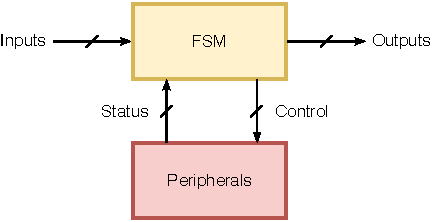
\includegraphics[width=.9\textwidth]{controller_generic}
  \end{column}
  \begin{column}{.48\textwidth}
    \begin{itemize}\small\itemsep3pt
      \item An FSM that interfaces with peripherals or supporting circuits.
      \item Outputs control external devices; status signals come back from peripherals; other inputs come from the environment.
      \item May have both Moore and Mealy outputs.
    \end{itemize}
  \end{column}
  \end{columns}
\end{frame}

\begin{frame}{Many Inputs, Many Outputs}
  \centering
  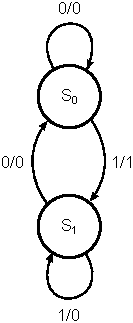
\includegraphics[height=.28\textheight]{controller-siso}\hspace{6mm}
  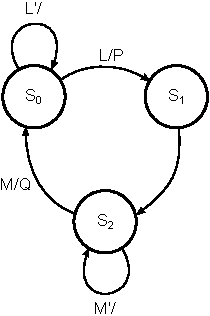
\includegraphics[height=.28\textheight]{controller-mimo}\hspace{6mm}
  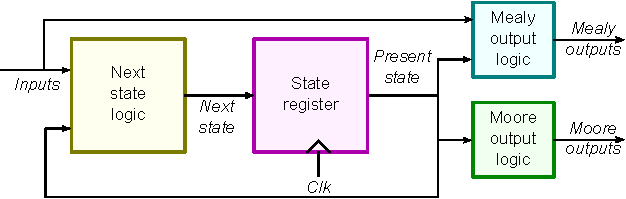
\includegraphics[height=.2\textheight]{fsm_mooremealy}
  \begin{itemize}\small\itemsep3pt
    \item In multi-input diagrams, arrows are labelled with Boolean conditions on named signals instead of 0 and 1.
    \item Use Moore outputs where possible (easy to analyse). Use Mealy outputs where a pulse is needed without a dedicated state. Mixing both can simplify the design.
  \end{itemize}
\end{frame}

%===============================================================================
\section{Vending Machine}
%===============================================================================

\begin{frame}{Vending Machine Controller}
  \begin{columns}[c]
  \begin{column}{.45\textwidth}
    \centering
    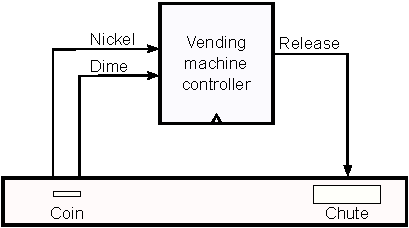
\includegraphics[width=.9\textwidth]{vending_top}
  \end{column}
  \begin{column}{.53\textwidth}
    \begin{itemize}\small\itemsep3pt
      \item One coin slot; nickels (5 cents) and dimes (10 cents), one at a time. A sensor identifies the coin.
      \item Releases the product at 15 cents. No change: two dimes lose 5 cents.
      \item Inputs $N$, $D$ (both 1 never occurs); output $Release$.
    \end{itemize}
    \centering\scriptsize
    \begin{tabular}{@{}cccc@{}}
      \textit{Penny} & \textit{Nickel} & \textit{Dime} & \textit{Quarter} \\
      
\includegraphics[width=8mm]{us-penny-104px} & 
\includegraphics[width=9mm]{us-nickel-116px} & 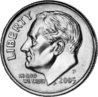
\includegraphics[width=7.5mm]{us-dime-98px} & 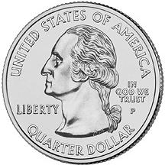
\includegraphics[width=10mm]{us-quarter-165px} \\
      1\textcent & 5\textcent & 10\textcent & 25\textcent \\
    \end{tabular}
  \end{column}
  \end{columns}
\end{frame}

\begin{frame}{Moore Vending Machine: State Diagram}
  \begin{columns}[c]
  \begin{column}{.3\textwidth}
    \centering
    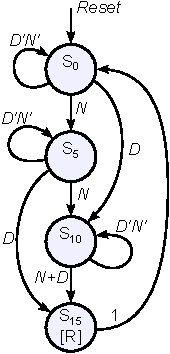
\includegraphics[height=.62\textheight]{vending_moore_sd}
  \end{column}
  \begin{column}{.68\textwidth}
    \begin{itemize}\small\itemsep3pt
      \item $S_0$: no money; $S_5$, $S_{10}$, $S_{15}$: that amount received.
      \item A nickel moves forward one state; a dime moves two. No coin: stay (loop $D'N'$).
      \item In $S_{15}$ the machine asserts $Release$, then returns to $S_0$ unconditionally (arrow labelled 1).
      \item Arrows carry Boolean conditions such as $D'N'$, $N + D$, $D$.
    \end{itemize}
  \end{column}
  \end{columns}
\end{frame}

\begin{frame}{Moore Vending Machine: State Table}
  \begin{columns}[c]
  \begin{column}{.5\textwidth}
    \centering\tiny\striped
    \begin{tabular}{@{}c|cc|c|c@{}}
      \toprule
      State & $D$ & $N$ & Next & $Release$ \\
      \midrule
      $S_0$ & 0&0 & $S_0$ & 0 \\ & 0&1 & $S_5$ & 0 \\ & 1&0 & $S_{10}$ & 0 \\ & 1&1 & $\times$ & 0 \\
      $S_5$ & 0&0 & $S_5$ & 0 \\ & 0&1 & $S_{10}$ & 0 \\ & 1&0 & $S_{15}$ & 0 \\ & 1&1 & $\times$ & 0 \\
      $S_{10}$ & 0&0 & $S_{10}$ & 0 \\ & 0&1 & $S_{15}$ & 0 \\ & 1&0 & $S_{15}$ & 0 \\ & 1&1 & $\times$ & 0 \\
      $S_{15}$ & $\times$&$\times$ & $S_0$ & 1 \\
      \bottomrule
    \end{tabular}
  \end{column}
  \begin{column}{.48\textwidth}
    \begin{itemize}\small\itemsep3pt
      \item $DN = 11$ is impossible: don't cares.
      \item Binary encoding: $S_0 = 00$, $S_5 = 01$, $S_{10} = 10$, $S_{15} = 11$.
    \end{itemize}
    \small
    $D_1 = Q_1'D + Q_1Q_0' + Q_1'Q_0N$\\
    $D_0 = Q_0'N + Q_1'Q_0N' + Q_1Q_0'D$\\
    $R = Q_1Q_0$
  \end{column}
  \end{columns}
\end{frame}

\begin{frame}{Moore Vending Machine: Circuit}
  \centering
  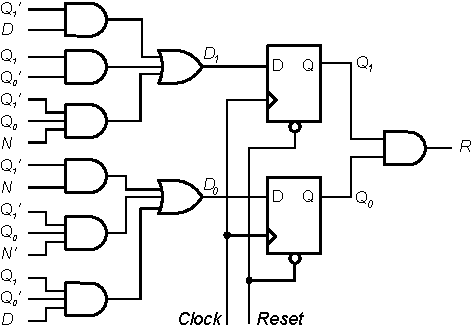
\includegraphics[height=.62\textheight]{vending_moore_kmap_sc}
  \begin{itemize}\small
    \item Two flip-flops with next-state logic built from the equations; $R$ comes straight from the state bits.
  \end{itemize}
\end{frame}

\begin{frame}{Mealy Vending Machine}
  \begin{columns}[c]
  \begin{column}{.5\textwidth}
    \centering
    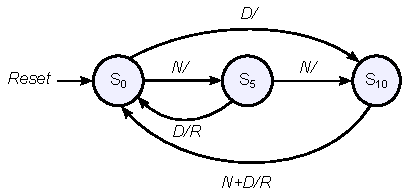
\includegraphics[width=.9\textwidth]{vending_mealy_kmap_sd}
    \begin{itemize}\small\itemsep3pt
      \item No $S_{15}$ state: $R$ is produced during the transition from $S_5$ or $S_{10}$ back to $S_0$.
      \item Three states, encoding $S_0 = 00$, $S_5 = 01$, $S_{10} = 10$.
    \end{itemize}
  \end{column}
  \begin{column}{.48\textwidth}
    \small
    $D_1 = Q_0N + Q_1'Q_0'D + Q_1D'N'$\\
    $D_0 = Q_1'Q_0'N + Q_0D'N'$\\
    $R = Q_0D + Q_1N + Q_1D$
    \begin{itemize}\small\itemsep3pt
      \item Literals: 20 against the Moore version's 17, mostly in $R$ (six literals, since it depends on the inputs as well as the state). One fewer state, but here that does not pay for the extra output logic, so the implementation is skipped.
    \end{itemize}
  \end{column}
  \end{columns}
\end{frame}

%===============================================================================
\section{One-Hot Encoding}
%===============================================================================

\begin{frame}{One-Hot Moore Vending Machine}
  \begin{columns}[c]
  \begin{column}{.5\textwidth}
    \begin{itemize}\small\itemsep3pt
      \item One flip-flop per state; only the current state's flip-flop is ``hot''.
      \item $S_0 = 0001$, $S_5 = 0010$, $S_{10} = 0100$, $S_{15} = 1000$.
      \item Each \alert{incoming arrow} gives one term: originating state AND the arrow's condition. No Boolean reduction needed.
    \end{itemize}
    \centering
    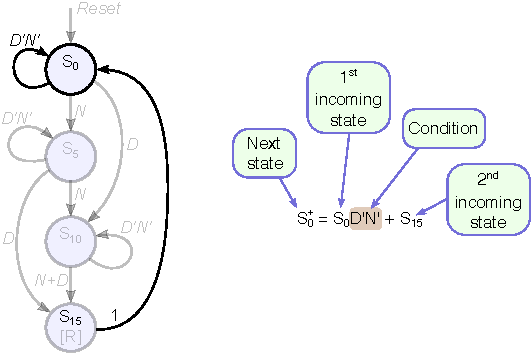
\includegraphics[width=.8\textwidth]{derive_1hot}
  \end{column}
  \begin{column}{.48\textwidth}
    \small
    $S_0^+ = S_0D'N' + S_{15}$\\
    $S_5^+ = S_0N + S_5D'N'$\\
    $S_{10}^+ = S_0D + S_5N + S_{10}D'N'$\\
    $S_{15}^+ = S_5D + S_{10}N + S_{10}D$\\[2mm]
    $R = S_{15}$
  \end{column}
  \end{columns}
\end{frame}

\begin{frame}{One-Hot Circuit and Reset}
  \begin{columns}[c]
  \begin{column}{.5\textwidth}
    \centering
    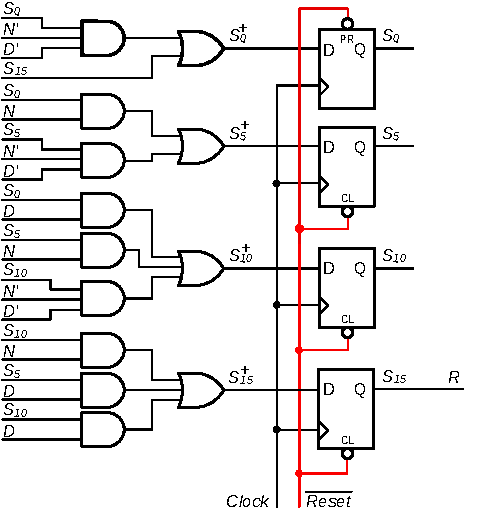
\includegraphics[height=.62\textheight]{vending_oh_sc}
  \end{column}
  \begin{column}{.48\textwidth}
    \begin{itemize}\small\itemsep3pt
      \item $\overline{Reset}$ drives the preset of the first flip-flop and the clear of the others, forcing $S_0$.
      \item One-hot logic is not limited to four input variables and is easy to extend.
    \end{itemize}
  \end{column}
  \end{columns}
\end{frame}

\begin{frame}{Automatic Reset: Power-On Reset}
  \centering
  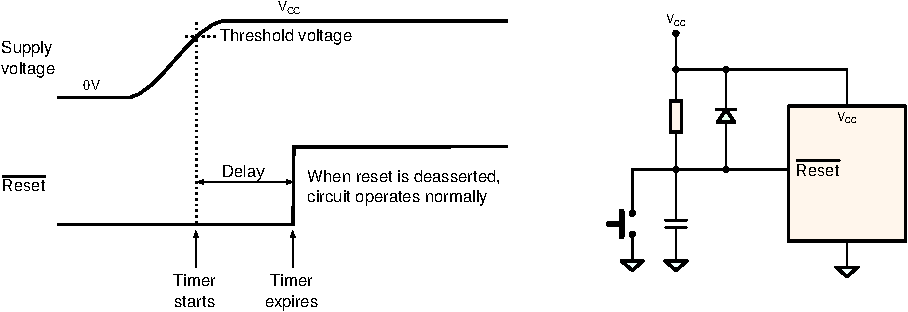
\includegraphics[width=.65\textwidth]{por_td}
  \begin{itemize}\small\itemsep3pt
    \item A real system must start without human help. A \alert{power-on-reset} circuit holds reset low while the supply rises. A timer starts when the supply crosses a threshold; POR is released high only when the timer expires.
    \item Until then all flip-flops are forced to the initial state.
  \end{itemize}
\end{frame}

\begin{frame}{Automatic Reset: Inverted First Flip-Flop}
  \begin{columns}[c]
  \begin{column}{.5\textwidth}
    \begin{itemize}\small\itemsep3pt
      \item In CPLDs and FPGAs all flip-flops power up as 0. For a highly encoded FSM, all-zero is a fine initial state; for one-hot it is the ``none-hot'' state.
      \item Fix: use \alert{negative logic} on the first flip-flop (an inverter at its input and output). Then all-zeros means $S_0$.
    \end{itemize}
    \centering\small\striped
    \begin{tabular}{@{}lcc@{}}
      \toprule
      State & Actual FFs & Reads as \\
      \midrule
      $S_0$ & 0000 & 0001 \\ $S_5$ & 0011 & 0010 \\ $S_{10}$ & 0101 & 0100 \\ $S_{15}$ & 1001 & 1000 \\
      \bottomrule
    \end{tabular}
  \end{column}
  \begin{column}{.48\textwidth}
    \centering
    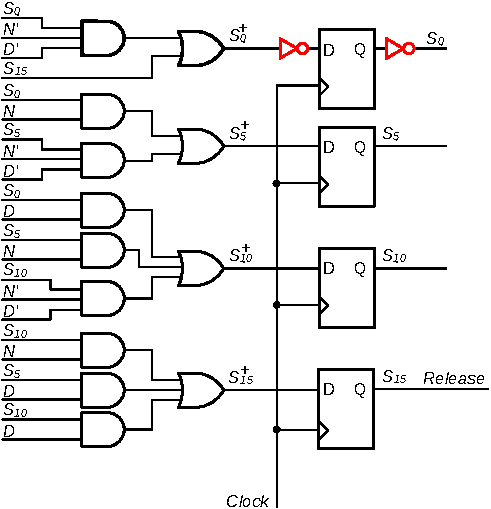
\includegraphics[height=.6\textheight]{vending_oh_sc_f1}
  \end{column}
  \end{columns}
\end{frame}

%===============================================================================
\section{Zebra Crossing}
%===============================================================================

\begin{frame}{Zebra Crossing Controller}
  \begin{columns}[c]
  \begin{column}{.45\textwidth}
    \centering
    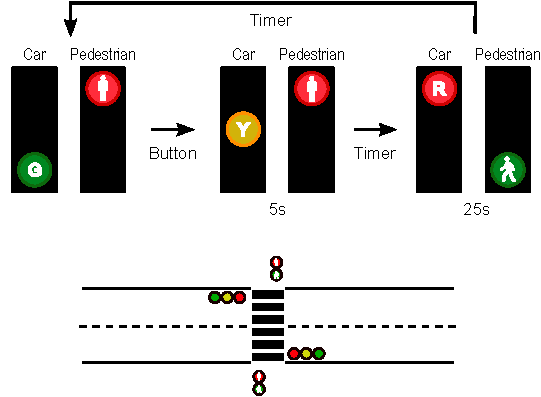
\includegraphics[width=\textwidth]{zebra_overview}
  \end{column}
  \begin{column}{.53\textwidth}
    \begin{itemize}\small\itemsep3pt
      \item Adds a \alert{timer subsystem}: the controller starts the timer with a control signal and waits for its status signal.
      \item Car lights $R, Y, G$; pedestrian lights $W$ (walk), $D$ (don't walk); input $B$ (button).
      \item Cars have right of way by default. A press gives 5 s of yellow, then 25 s of red/walk.
    \end{itemize}
    \centering\scriptsize\striped
    \begin{tabular}{@{}lccc@{}}
      \toprule
      State & Car & Pedestrian & Period \\
      \midrule
      Initial & Green & Don't walk & Infinite \\ Transition & Yellow & Don't walk & 5 s \\ Safe to walk & Red & Walk & 25 s \\
      \bottomrule
    \end{tabular}
  \end{column}
  \end{columns}
\end{frame}

\begin{frame}{Zebra Crossing: Interfaces and Timer}
  \begin{columns}[c]
  \begin{column}{.4\textwidth}
    \centering
    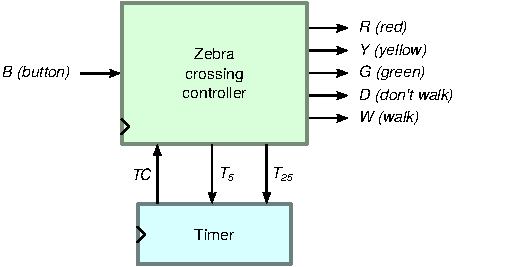
\includegraphics[width=.95\textwidth]{zebra_top}
  \end{column}
  \begin{column}{.58\textwidth}
    \centering
    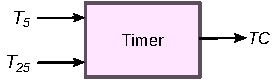
\includegraphics[height=.12\textheight]{zebra_timer_top}\hspace{3mm}
    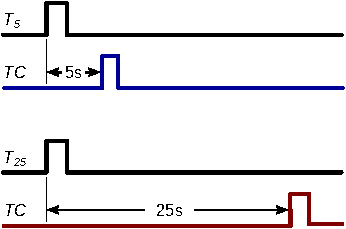
\includegraphics[height=.18\textheight]{zebra_timing}
    \begin{itemize}\small\itemsep3pt
      \item The controller sends $T_5$ or $T_{25}$ to the timer. After 5 s or 25 s the timer asserts \textit{TC} (terminal count).
      \item The timer is internal; its signals are not visible outside.
    \end{itemize}
  \end{column}
  \end{columns}
\end{frame}

\begin{frame}{First-Cut Moore Design}
  \begin{columns}[c]
  \begin{column}{.45\textwidth}
    \centering
    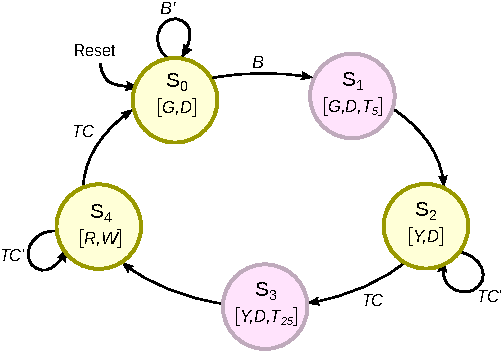
\includegraphics[width=\textwidth]{zebra_moore_sd}
  \end{column}
  \begin{column}{.53\textwidth}
    \begin{itemize}\small\itemsep3pt
      \item $S_0$: $G$ and $D$ on; wait for $B = 1$.
      \item $S_1$: one cycle that asserts $T_5$ to trigger the timer.
      \item $S_2$: yellow for 5 s; wait for $TC$.
      \item $S_3$: one cycle that asserts $T_{25}$.
      \item $S_4$: red and walk for 25 s; on $TC$, back to $S_0$.
      \item Two states exist only to trigger the timer: in a pure Moore machine an output must live inside a state.
    \end{itemize}
  \end{column}
  \end{columns}
\end{frame}

\begin{frame}{The Timer Module}
  \begin{columns}[c]
  \begin{column}{.5\textwidth}
    \centering
    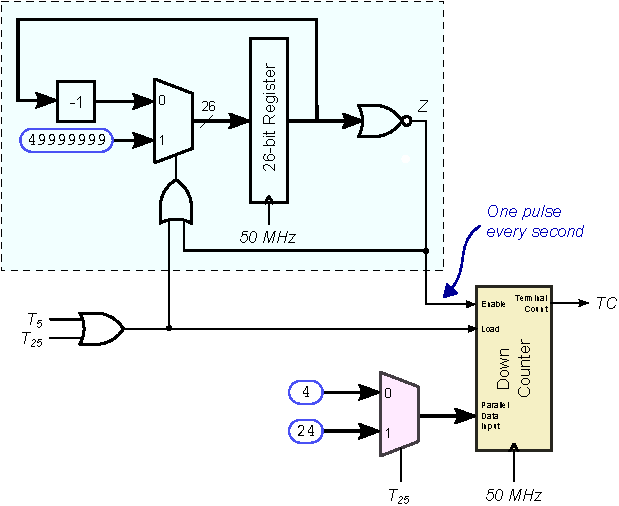
\includegraphics[width=\textwidth]{zebra_timer_sc}
  \end{column}
  \begin{column}{.48\textwidth}
    \begin{itemize}\small\itemsep3pt
      \item A 1 Hz timing reference (the prescaler of Section 11.4.4) pulses $Z$ once per second. At 50 MHz it counts down from 49,999,999.
      \item A 5-bit down-counter with load and enable counts seconds; loaded with 4 or 24 when $T_5$ or $T_{25}$ arrives.
      \item Loading $n$ gives an $(n+1)$-second delay, because \textit{TC} is seen on the clock after the count reaches 0.
    \end{itemize}
  \end{column}
  \end{columns}
\end{frame}

\begin{frame}{Improved Design: Mixed Moore and Mealy}
  \begin{columns}[c]
  \begin{column}{.4\textwidth}
    \centering
    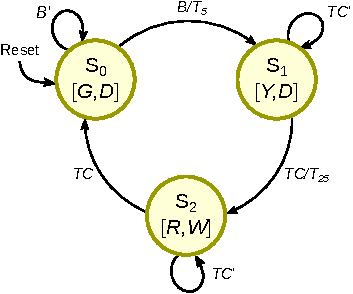
\includegraphics[width=\textwidth]{zebra_mealy_sd}
  \end{column}
  \begin{column}{.58\textwidth}
    \centering\tiny\striped
    \begin{tabular}{@{}c|cc|c|ccccccc@{}}
      \toprule
      State & $B$ & $TC$ & Next & $D$ & $W$ & $R$ & $Y$ & $G$ & $T_5$ & $T_{25}$ \\
      \midrule
      $S_0$ & 0 & $\times$ & $S_0$ & 1&0&0&0&1&0&0 \\
      $S_0$ & 1 & $\times$ & $S_1$ & 1&0&0&0&1&1&0 \\
      $S_1$ & $\times$ & 0 & $S_1$ & 1&0&0&1&0&0&0 \\
      $S_1$ & $\times$ & 1 & $S_2$ & 1&0&0&1&0&0&1 \\
      $S_2$ & $\times$ & 0 & $S_2$ & 0&1&1&0&0&0&0 \\
      $S_2$ & $\times$ & 1 & $S_0$ & 0&1&1&0&0&0&0 \\
      \bottomrule
    \end{tabular}
    \begin{itemize}\small\itemsep2pt
      \item Triggering the timer on a \alert{transition} (Mealy output) removes the two trigger states: three states instead of five.
    \end{itemize}
  \end{column}
  \end{columns}
\end{frame}

\begin{frame}{Zebra Crossing: Equations and Circuit}
  \begin{columns}[c]
  \begin{column}{.4\textwidth}
    \small One-hot next state:\\
    $S_0^+ = S_0B' + S_2TC$\\
    $S_1^+ = S_0B + S_1TC'$\\
    $S_2^+ = S_1TC + S_2TC'$\\[2mm]
    Moore outputs: $D = S_0 + S_1$, $W = R = S_2$, $Y = S_1$, $G = S_0$.\\[2mm]
    Mealy outputs: $T_5 = S_0B$, $T_{25} = S_1TC$.
  \end{column}
  \begin{column}{.58\textwidth}
    \centering
    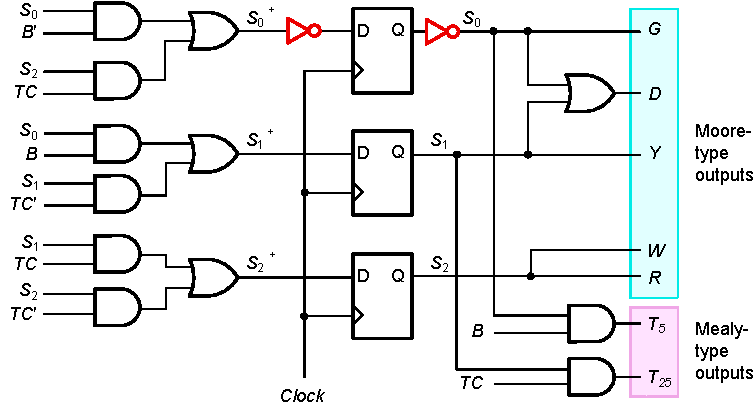
\includegraphics[width=\textwidth]{zebra_1h_sc}
  \end{column}
  \end{columns}
\end{frame}

%===============================================================================
\section{Traffic Light}
%===============================================================================

\begin{frame}{Traffic Light Controller}
  \begin{columns}[c]
  \begin{column}{.45\textwidth}
    \centering
    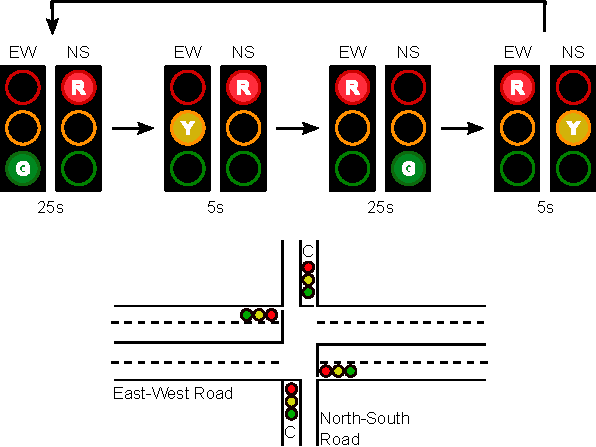
\includegraphics[width=\textwidth]{tlc_overview}
  \end{column}
  \begin{column}{.53\textwidth}
    \begin{itemize}\small\itemsep3pt
      \item Reuses the timer idea of the zebra crossing, with more states and timed phases.
      \item East-West has priority (green by default); North-South has a car sensor $C$.
      \item A car on North-South triggers: EW yellow 5 s, then NS green (at most 25 s), then NS yellow 5 s, then back to EW green.
    \end{itemize}
    \centering\scriptsize\striped
    \begin{tabular}{@{}lccl@{}}
      \toprule
      State & EW & NS & Delay \\
      \midrule
      $S_0$ & Green & Red & $\ge 25$ s while $C = 0$ \\ $S_1$ & Yellow & Red & 5 s \\ $S_2$ & Red & Green & $\le 25$ s \\ $S_3$ & Red & Yellow & 5 s \\
      \bottomrule
    \end{tabular}
  \end{column}
  \end{columns}
\end{frame}

\begin{frame}{Traffic Light: Architecture and State Diagram}
  \begin{columns}[c]
  \begin{column}{.5\textwidth}
    \centering
    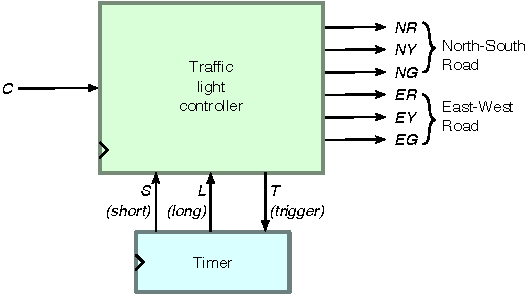
\includegraphics[height=.22\textheight]{tlc_top}\\[2mm]
    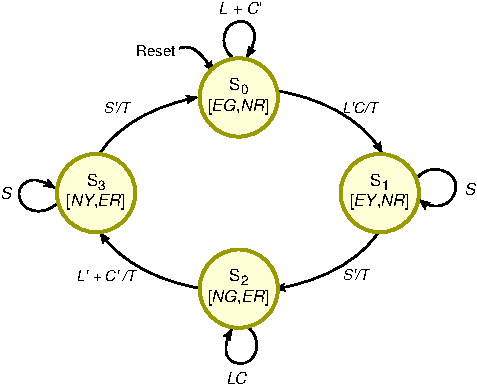
\includegraphics[height=.3\textheight]{tlc_sd}
  \end{column}
  \begin{column}{.48\textwidth}
    \begin{itemize}\small\itemsep3pt
      \item Inputs: $C$ (car sensor), $S$ (short timer), $L$ (long timer). Outputs: six lights and $T$ (trigger).
      \item $S_0$: exit on $L'C$ (long timer expired and car present): at least 25 s.
      \item $S_1$: stay while $S = 1$; when $S = 0$ trigger the timer and go to $S_2$.
      \item $S_2$: stay only while $L$ and $C$ are both 1; otherwise go to $S_3$ and trigger the timer.
      \item $S_3$: stay while $S = 1$, then return to $S_0$.
    \end{itemize}
  \end{column}
  \end{columns}
\end{frame}

\begin{frame}{Traffic Light Timer Subsystem}
  \begin{columns}[c]
  \begin{column}{.5\textwidth}
    \centering
    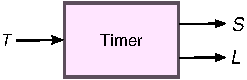
\includegraphics[height=.1\textheight]{tlc_timer_top}\hspace{3mm}
    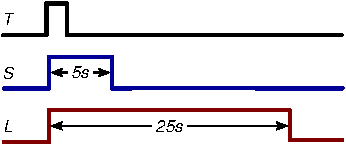
\includegraphics[height=.12\textheight]{tlc_timing}\\[3mm]
    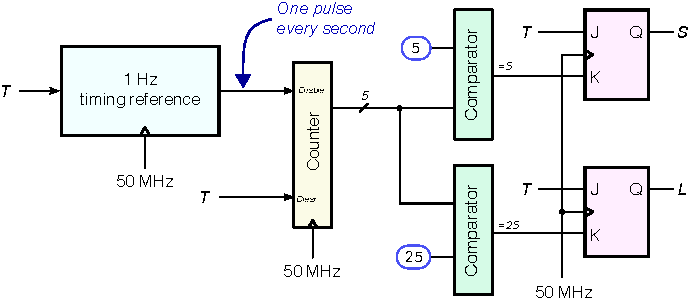
\includegraphics[width=\textwidth]{tlc_timer_jk_sc}
  \end{column}
  \begin{column}{.48\textwidth}
    \begin{itemize}\small\itemsep3pt
      \item Trigger $T$ sets both outputs $S$ and $L$ high; they go low after 5 s and 25 s.
      \item Library version: a counter, two comparators and two JK flip-flops. $T$ resets the counter and the 1 Hz reference; the comparators detect 5 and 25 and reset the flip-flops.
    \end{itemize}
  \end{column}
  \end{columns}
\end{frame}

\begin{frame}{Gate-Level Timer}
  \begin{columns}[c]
  \begin{column}{.5\textwidth}
    \centering
    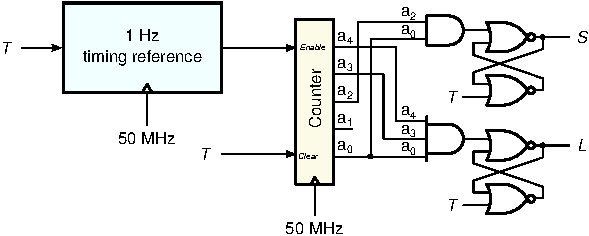
\includegraphics[width=\textwidth]{tlc_timer_sc}
  \end{column}
  \begin{column}{.48\textwidth}
    \begin{itemize}\small\itemsep3pt
      \item Smaller version: $S$ and $L$ come from SR latches set by $T$.
      \item Because 5 and 25 are fixed, a gate detects them cheaply: $a_2 a_0$ detects $xx1x1_2$, and $5 = 00101_2$ is the first such value reached.
      \item $a_4a_3a_0$ detects $11xx1_2$, and $25 = 11001_2$ is the first match.
      \item Each AND output resets its latch.
    \end{itemize}
  \end{column}
  \end{columns}
\end{frame}

\begin{frame}{Traffic Light: One-Hot Implementation}
  \begin{columns}[c]
  \begin{column}{.4\textwidth}
    \small One-hot states $S_0 = 0001$ to $S_3 = 1000$.
    \begin{align*}
      S_0^+ &= S_0(L + C') + S_3S' \\
      S_1^+ &= S_0L'C + S_1S \\
      S_2^+ &= S_1S' + S_2LC \\
      S_3^+ &= S_2(L' + C') + S_3S
    \end{align*}
    \footnotesize
    $T = S_0L'C + S_1S' + S_2(L'+C') + S_3S'$\\
    $EG = S_0$, $EY = S_1$, $ER = S_2 + S_3$\\
    $NG = S_2$, $NY = S_3$, $NR = S_0 + S_1$
  \end{column}
  \begin{column}{.58\textwidth}
    \centering
    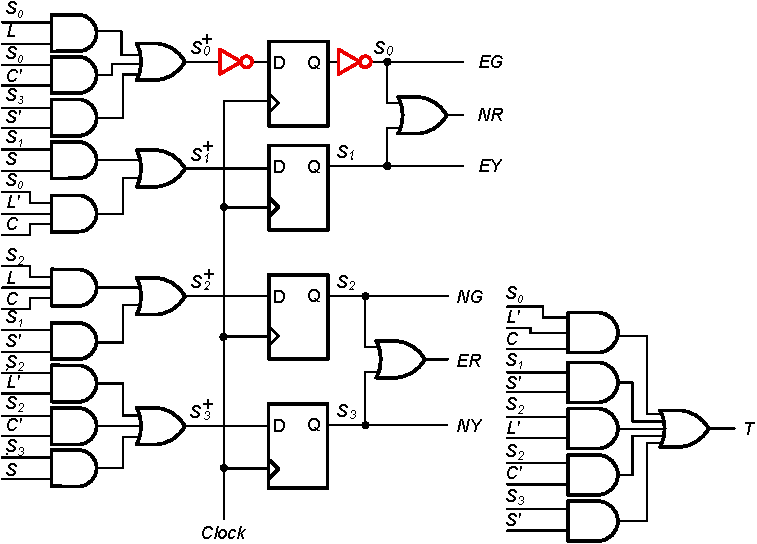
\includegraphics[width=.95\textwidth]{tlc_1h_sc}
  \end{column}
  \end{columns}
\end{frame}

\begin{frame}{Back to the Opening Question}
  \begin{block}{Vending machine states and inputs}
    \small \textbf{States}: the amount received so far ($S_0$, $S_5$, $S_{10}$, and a release state $S_{15}$ in the Moore design).\\
    \textbf{Inputs}: $N$ (nickel) and $D$ (dime); $ND = 11$ is impossible.\\
    \textbf{Transitions}: a nickel moves one step, a dime two; reaching 15 cents asserts $Release$ and returns to $S_0$. For a different price or coin set, add one state per reachable total.
  \end{block}
\end{frame}

%===============================================================================
\section{Summary}
%===============================================================================

\begin{frame}{Summary}
  \begin{itemize}\itemsep3pt\small
    \item A \alert{controller} is an FSM that sequences operations on something else: a timer, a peripheral, the lights.
    \item Here the controlled circuits are register-based blocks (counters, timers) and simple actuators: no data processing.
    \item Many controllers mix Moore outputs (stable, used as enables and selects) with Mealy outputs (reactive, used for pulses).
    \item Prescalers and divided clocks give a controller a slower timebase without complicating the state diagram.
    \item Always define a reset state; every reachable state needs a transition for every input combination.
  \end{itemize}
  \begin{block}{Looking ahead}
    Controllers can also work with \emph{datapaths}, the circuits that process data, and this scales up to complete processors. Chapter 16 introduces Verilog for describing all of this.
  \end{block}
\end{frame}

\end{document}
